\chapter{Patrones GoF}
\section{Patrones Creacionales}
\section{Patrones de Comportamiento}

\section{Patrones Estructurales}

\subsection{Patrón Proxy}

\subsubsection{Descripción}
El patron Proxy es un patrón que permite controlar el acceso a un objeto, esto  mediante una entidad intermediara, por lo cual se puede diferir el costo total de la creación de un objeto hasta que realmente necesitemos usarlo, buscando finalmente optimizar tanto el uso de recursos computacionales como los tiempos de carga.

Tiene como aplicación:

\begin{itemize}
	\item Un proxy remoto puede ocultar el hecho de que un objeto reside en un espacio de direcciones diferente.
	\item Un proxy virtual puede realizar optimizaciones, como crear un objeto a pedido.
	\item Los proxies de protección y referencias inteligentes permiten darle diferentes permisos de objetoa a los que así lo necesitan.
\end{itemize}

\paragraph{Estructura}

\begin{figure}[th!]
	\centering
	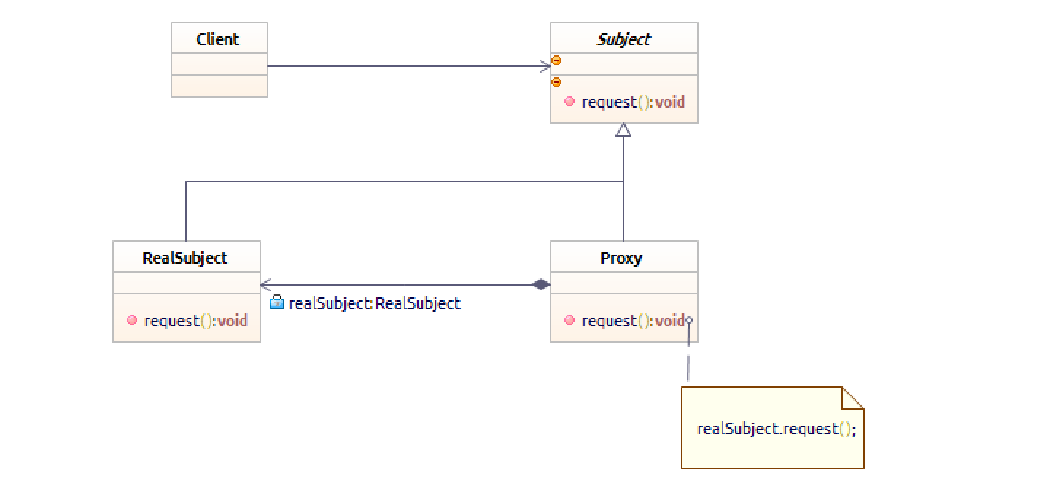
\includegraphics[width=.7\linewidth]{imganes/Patrones/estructura_Proxy}
	\caption{Estructura del patrón Proxy.}	
\end{figure}

\paragraph{Actores}

\begin{itemize}
	\item \texbf{Proxy}: Controla el acceso al sujeto real y puede ser responsable de crearlo y eliminarlo.
	\item \texbf{Sujeto}:Define la interfaz común para las clase SujetoReal y Proxy para que un Proxy se pueda usar en cualquier lugar donde se espere un SujetoReal.
	\item \texbf{Sujeto Real}:Define el objeto real al cual representa el Proxy.
\end{itemize}


\subsubsection{Caso de Uso}
